\documentclass[letterpaper,12pt]{book}

\usepackage[utf8]{inputenc} % Soporte para acentos
\usepackage[T1]{fontenc}    
\usepackage[spanish,mexico]{babel} % Español

% Soporte de símbolos adicionales (matemáticas)
\usepackage{amsmath}		
\usepackage{amssymb}		
\usepackage{amsfonts}
\usepackage{latexsym}

% Para inserción de imagenes
\usepackage[pdftex]{graphicx}
\usepackage{epstopdf}

% Algunos comandos y ambientes para tablas
\usepackage{tabularx}

% Para citas bibliograficas
\usepackage{cite}
\usepackage{hyperref}

\usepackage[lmargin=2cm,rmargin=2cm,top=2cm,bottom=2cm]{geometry}

% Información para el título
\title{Notas al Pie \\ 
	\vspace{1cm}Tablas de Contenidos \\ 
	\vspace{1cm}Índice de Figuras y Tablas\\
	\vspace{1cm}Bibliografía}
\author{J. Luis Torres}
\date{15 de junio de 2015}

% Indicamos una separación entre los párrafos
\parskip=3mm

% Eliminamos la sangría de los párrafos
\parindent=0mm

\begin{document}

\maketitle

\tableofcontents

\listoffigures

\listoftables

\chapter*{Prólogo}
\addcontentsline{toc}{chapter}{Prólogo}

En el futuro existirá un \emph{prólogo} en esta página.

\chapter{Gráficas sencillas con Maple 15}

\emph{Maple} es considerado un \emph{Sistema de Álgebra Computacional}, proporciona múltiples
funcionalidades al usuario entre las que se pueden listar las siguientes:

Las siguientes instrucciones nos permiten definir una función y generar su gráfica 
em Maple 15:

%Entorno que despliega tal cual símbolos y todo lo que introduzca
\begin{verbatim}
k:= x -> sin(x) + exp(cos(exp(x)));

plot(k(x), x=-10..4.5);
\end{verbatim}

Estas instrucciones nos permiten generar la gráfica que se muestra en la figura \ref{cap1f1}.

%begin{figure}[opcion] opcion= h! (here), t (top),b (bottom), p (page)
\begin{figure}[h!]
\centering
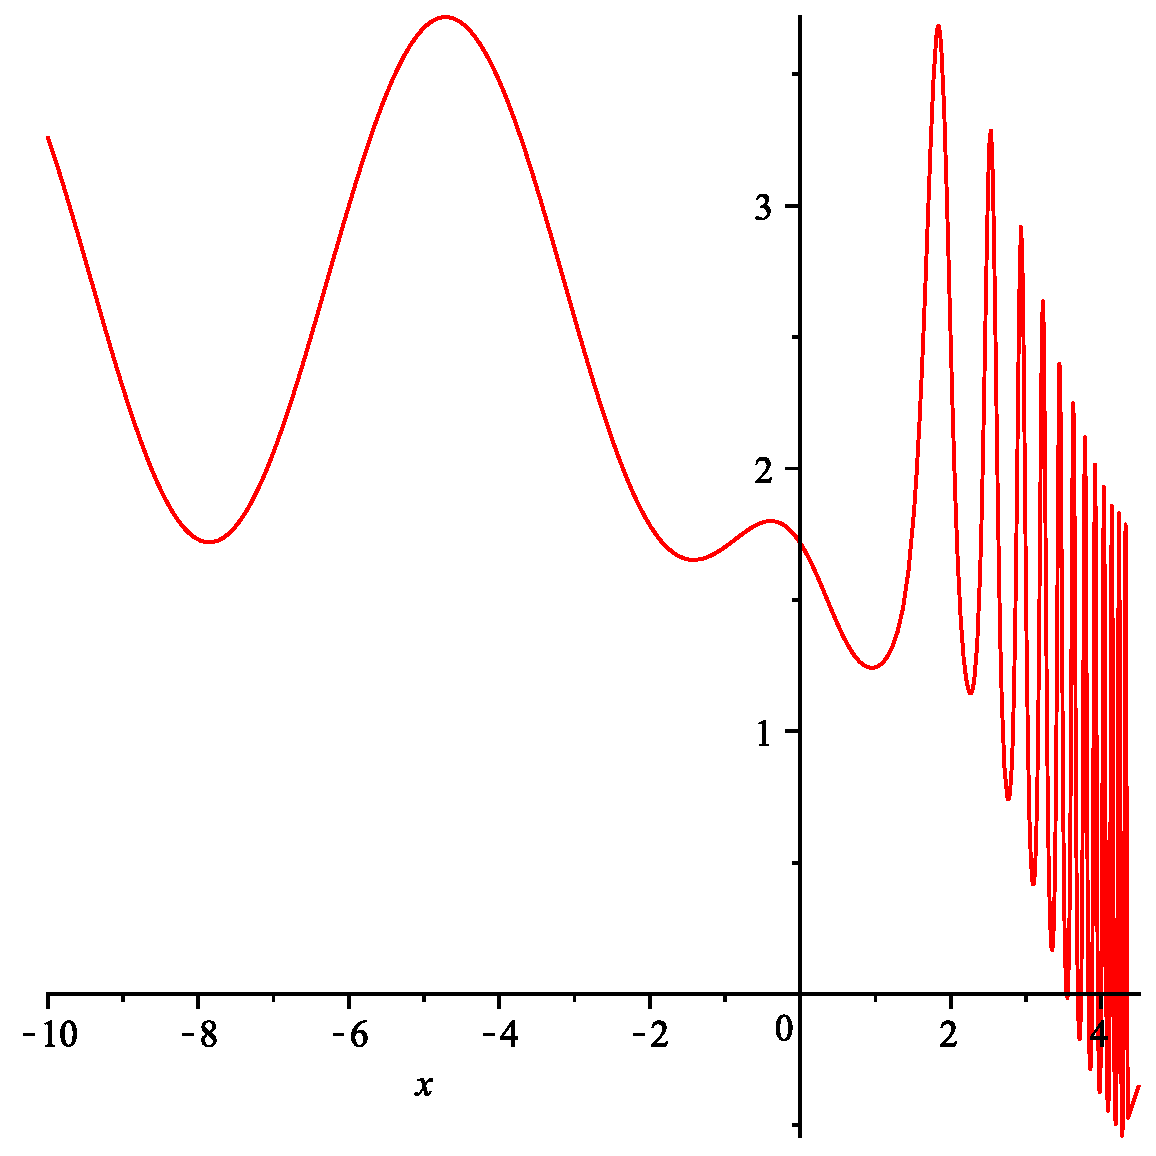
\includegraphics[scale=0.45]{grafica01.pdf}
\caption{Gráfica de $sen \left( x \right) +{{\rm e}^{\cos \left( {{\rm e}^{x}} \right) }}$}\label{cap1f1}
\end{figure}

\pagebreak

Veamos otro ejemplo:

Las siguientes instrucciones nos permiten generar la gráfica de la función 
$\displaystyle {x}^{4}\sin \left( {x}^{3} \right) -{x}^{3}\cos \left( {x}^{2}
 \right) +{x}^{2}\sin \left( x \right) -x$

\begin{verbatim}
plot(x^4*sin(x^3)-x^3*cos(x^2)+x^2*sin(x)-x, x = -1.8 .. 1.8);
\end{verbatim}

La gráfica se muestra en la figura \ref{cap1f2}.

\begin{figure}[h!]
\centering
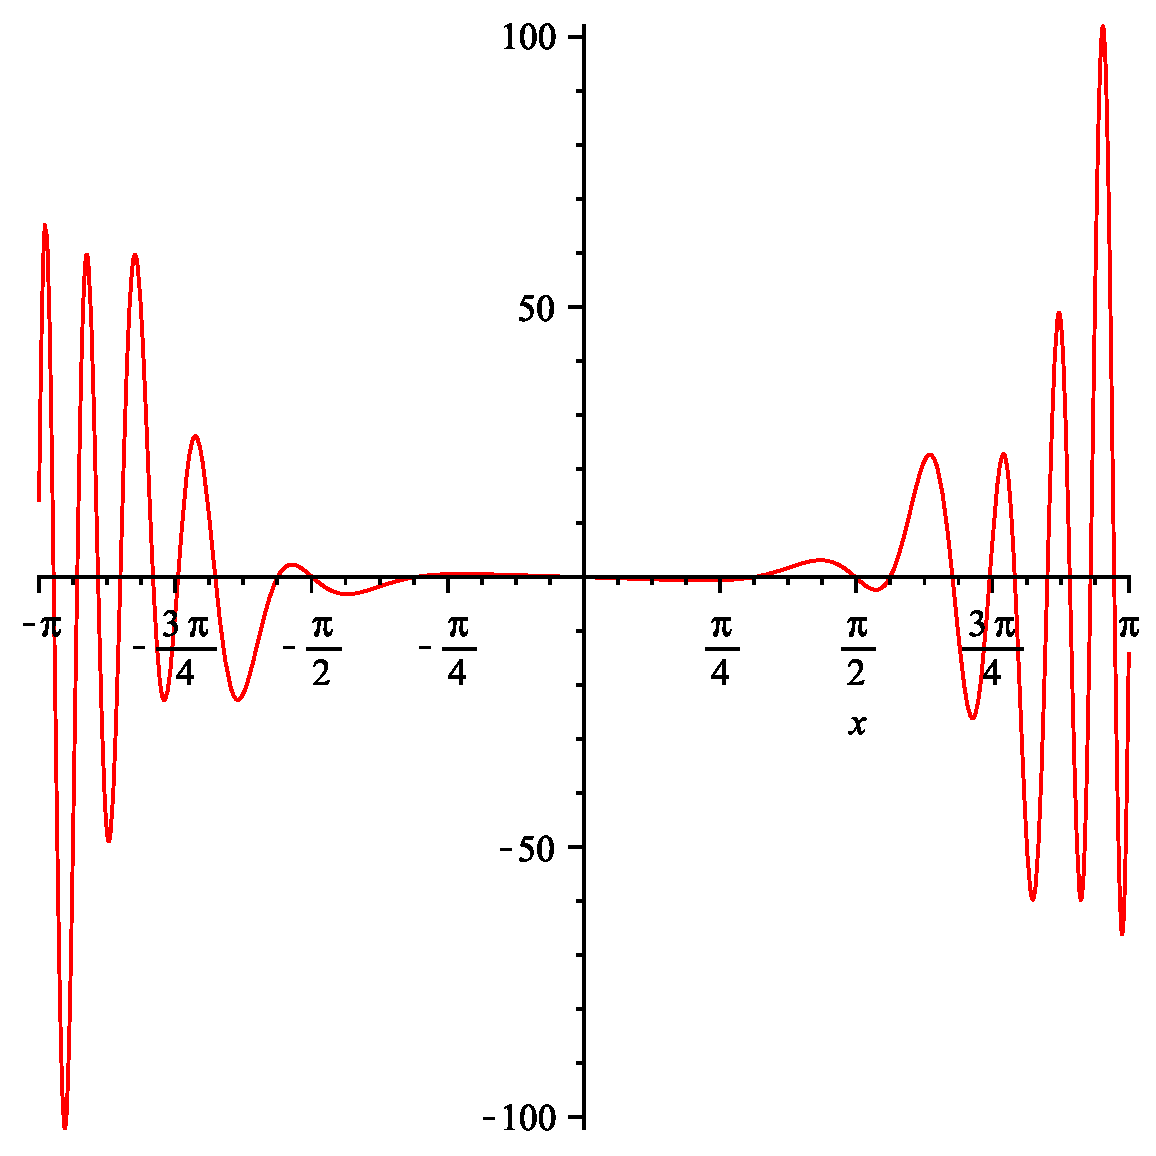
\includegraphics[scale=0.5]{grafica02.pdf}
\caption{Gráfica de ${x}^{4}\sin \left( {x}^{3} \right) -{x}^{3}\cos \left( {x}^{2}
 \right) +{x}^{2}\sin \left( x \right) -x$}\label{cap1f2}
\end{figure}

En la tabla \ref{tab:cap1t1} podemos consultar algunas instrucciones de \emph{Maple} que nos
permiten generar gráficas en dos dimensiones.

\begin{table}[h!]
	\caption{Instrucciones de Maple para gráficas en 2D}
	\begin{center}
		\begin{tabular}{|c|c|} \hline
			Instrucción & Tipo de gráfica generada \\ \hline
			plot() & Gráficas en 2D de funciones explicitas \\ \hline
			plot() & Gráficas en 2D de funciones paramétricas \\ \hline
			polarplot() & Gráficas en coordenadas polares \\ \hline
			implicitplot() & Gráficas implícitas en 2D \\ \hline
			complexplot() & Gráficas de expresiones complejas \\ \hline
			contourplot & Gráficas de contornos \\\hline
		\end{tabular}
	\end{center}
	\label{tab:cap1t1}
\end{table}

\chapter{Gráficas de Funciones con Discontinuidades}
\chaptermark{Gráficas con Discontinuidades}

Para poder generar gráficas de funciones de este tipo, la opción
\emph{discont=true} nos permite indicar a \emph{Maple} que éstas deben eliminarse de la
gráfica. La forma en la que incluimos esta opción es la siguiente:

\begin{verbatim}
plot(funcion(x), x = intervalo, {rango}, discont = true);
\end{verbatim}

Por ejemplo, la siguiente instrucción nos permite desplegar una gráfica de la 
función \emph{tan(x)}:

\begin{verbatim}
plot(tan(x), x = -10 .. 10, -50 .. 50, discont = true);
\end{verbatim}

La gráfica se puede ver en la figura \ref{cap2f1}.

\begin{figure}[h!]
\centering
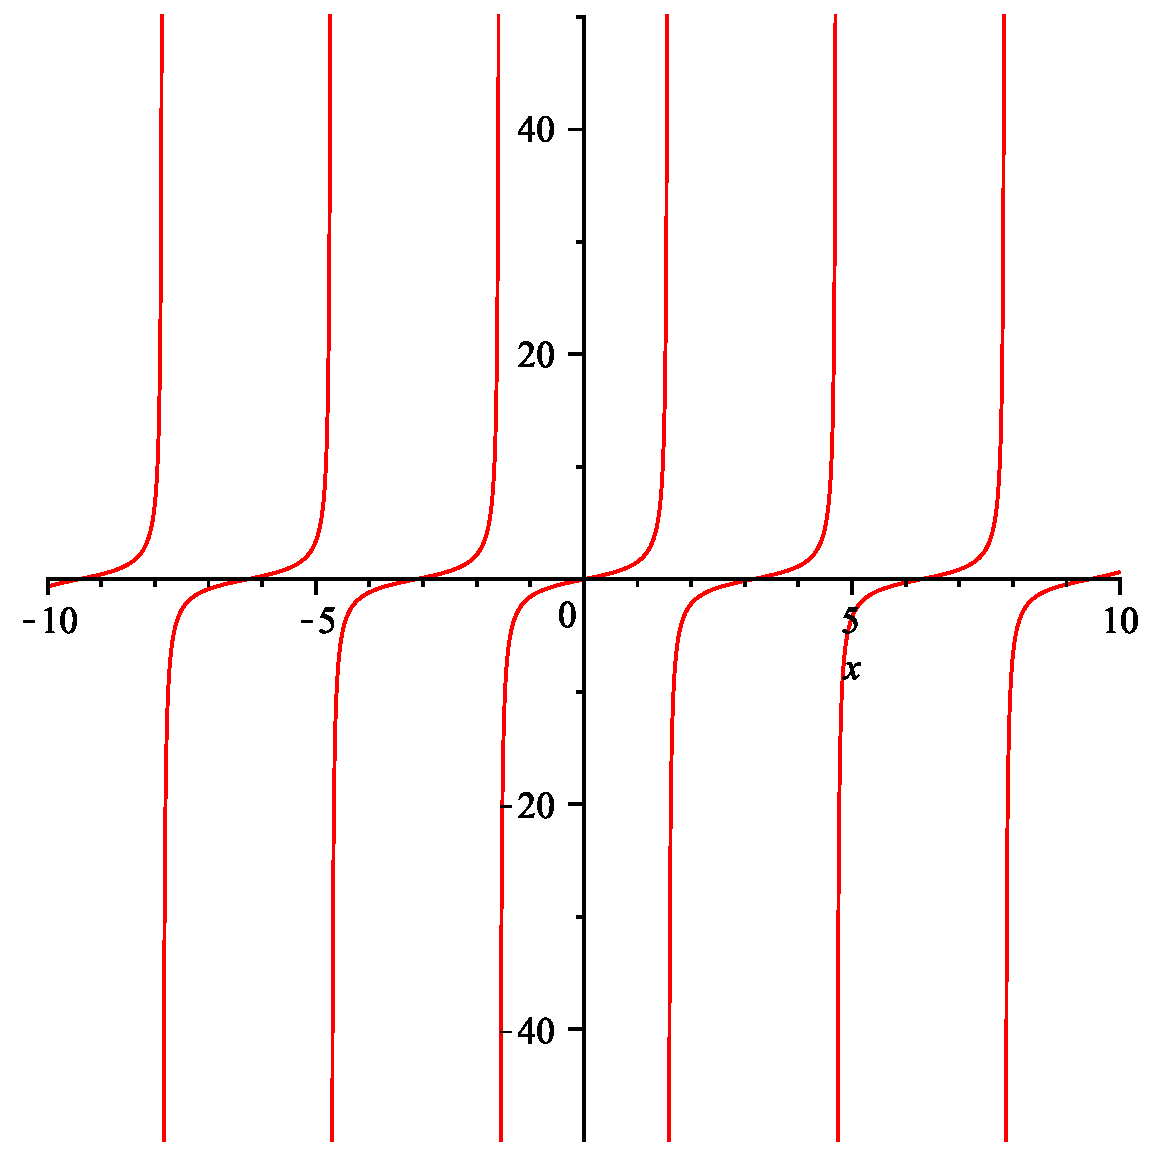
\includegraphics[scale=0.4]{grafica04.pdf}
\caption{Gráfica de $tan (x)$}\label{cap2f1}
\end{figure}

\chapter{Gráficas con Múltiples Funciones}

La siguiente instrucción nos permite incluir las gráficas de varias funciones en un mismo despliegue:

\begin{verbatim}
plot({x, cos(x), sin(x)}, x, color = [blue, brown, green]);
\end{verbatim}

La gráfica se puede observar en la figura \ref{cap3f1}.

\begin{figure}[h!]
\centering
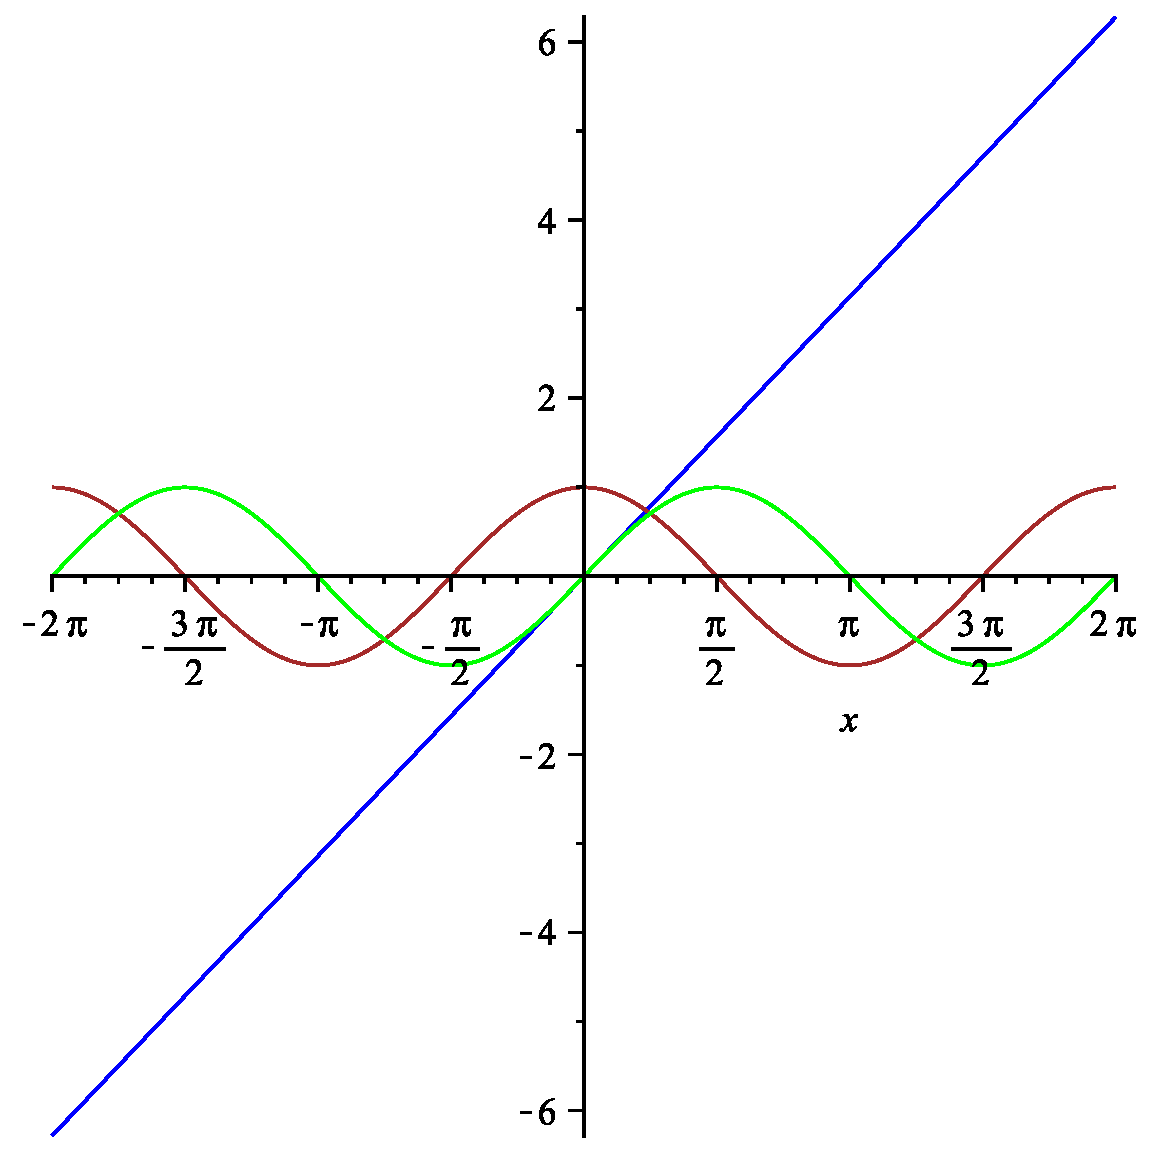
\includegraphics[scale=0.35]{grafica05.pdf}
\caption{Gráficas de $x$, $cos(x)$ y $sen(x)$}\label{cap3f1}
\end{figure}

\chapter{Gráficas de Contornos}

La siguiente instrucción nos permite desplegar una gráfica de contornos para una función de
$x$ y $y$, en el rectángulo indicado.

\begin{verbatim}
contourplot(sin(x)*y, x = -5 .. 5, y = -4 .. 4)
\end{verbatim}

Podemos ver la gráfica en la figura \ref{cap4f1}.

\begin{figure}[h!]
\centering
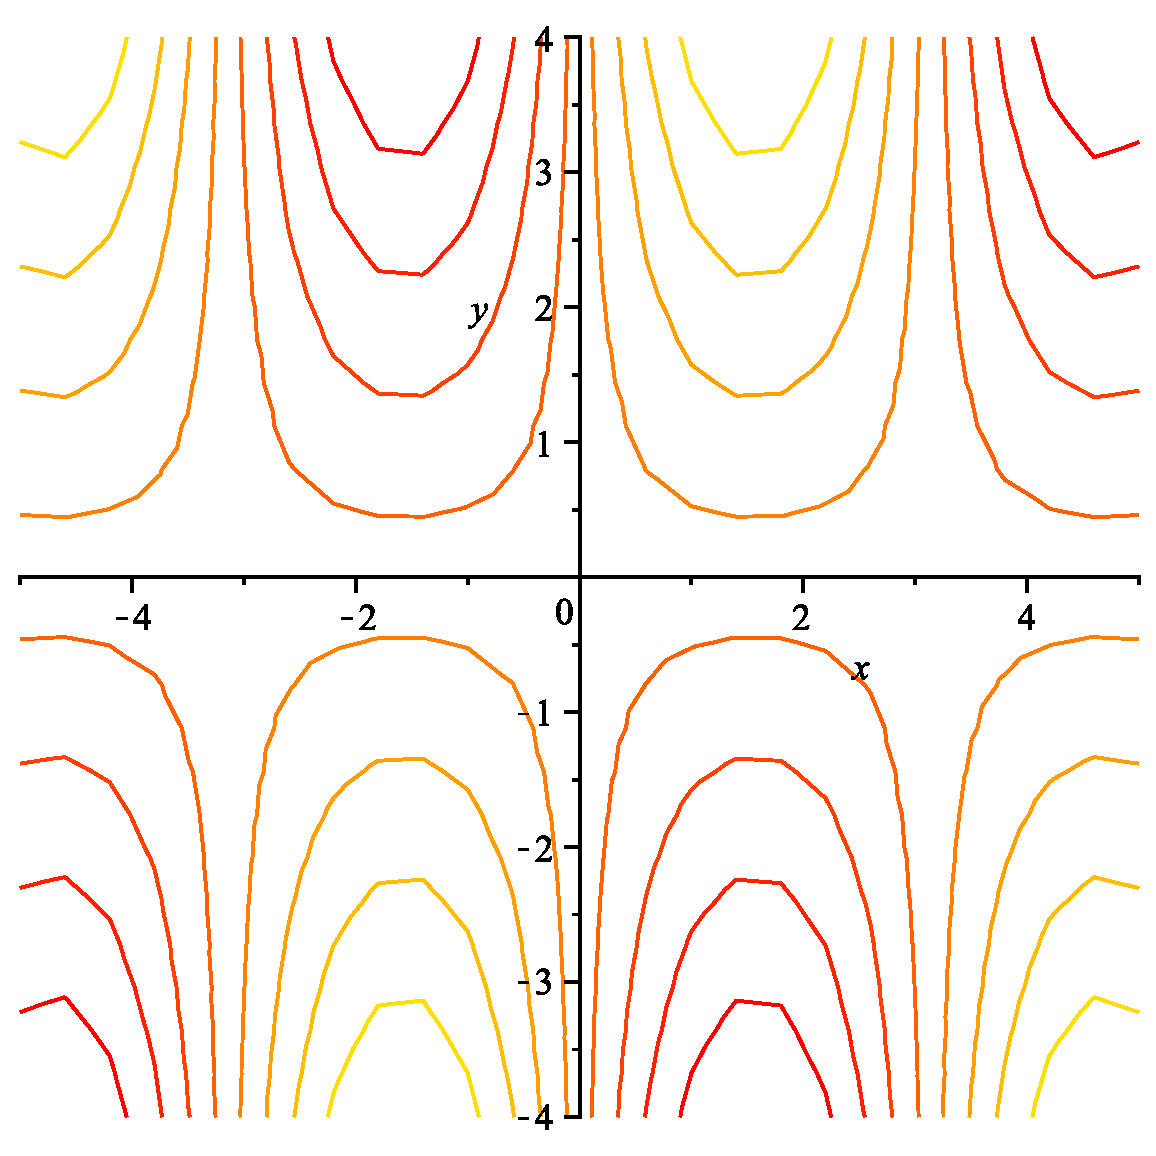
\includegraphics[scale=0.35]{grafica06.pdf}
\caption{Gráficas de contornos para $sen(x) \cdot y$}\label{cap4f1}
\end{figure}


\chapter{Gráficas en Coordenadas Polares}

Las siguientes instrucciones generarán una gráfica para 
$[t, sen()t]$ en el intervalo $\{0, 4\pi\}$, en coordenadas polares:

\begin{verbatim}
with(plots);
polarplot([t, sin(t), t = 0 .. 4*Pi], color = blue);
\end{verbatim}

La gráfica se puede apreciar en la figura \ref{cap5f1}.

\begin{figure}[h!]
\centering
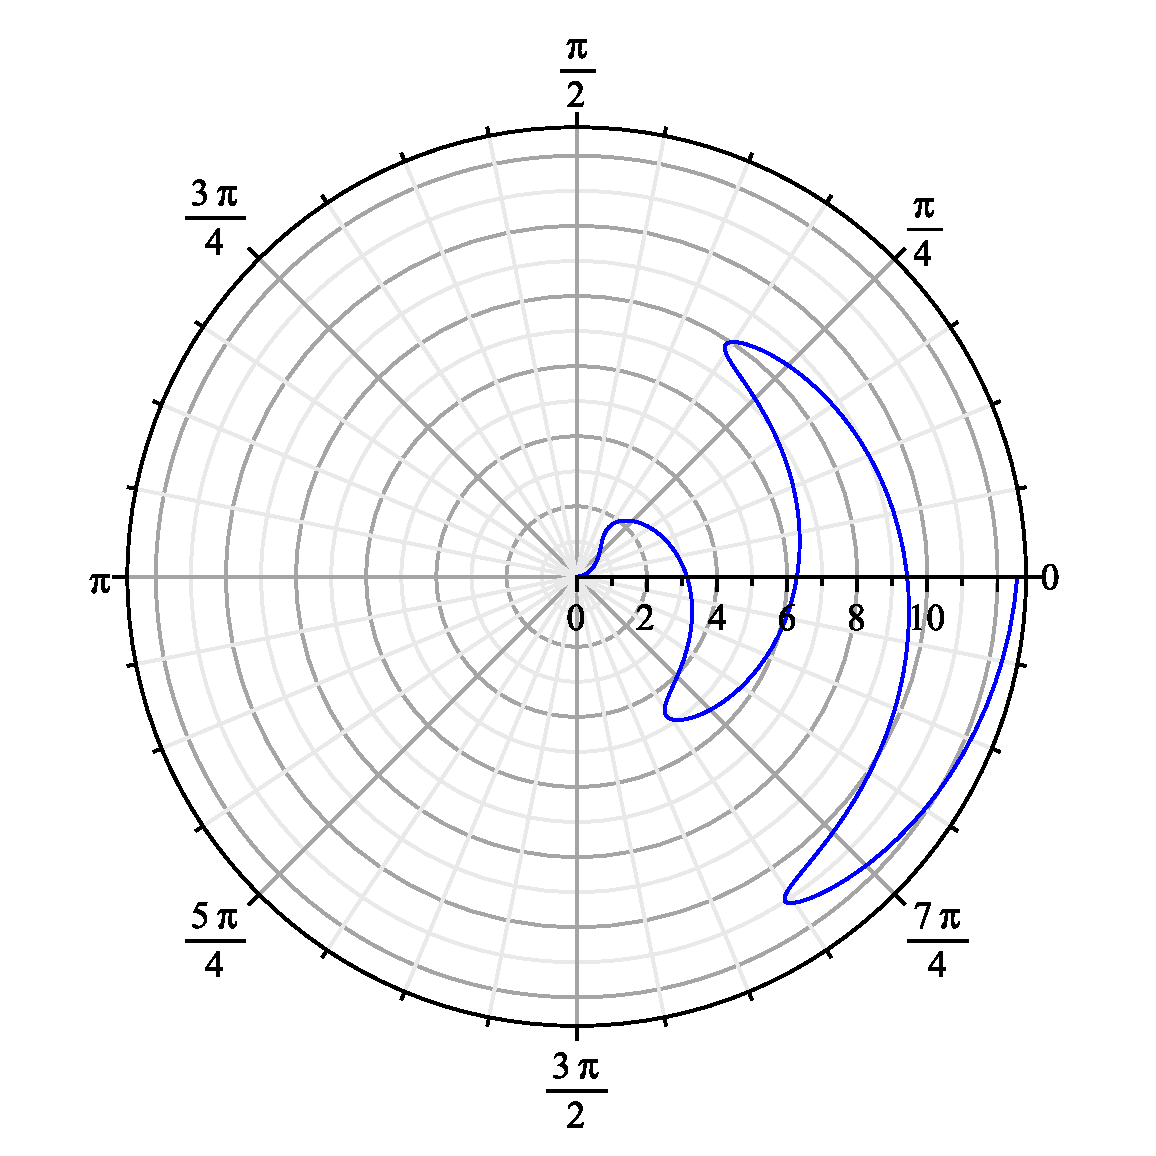
\includegraphics[scale=0.5]{grafica07.pdf}
\caption{Gráfica de $[t, sen()t]$ en coordenadas polares}\label{cap5f1}
\end{figure}

\chapter{Gráficas en 3D}

La siguiente instrucción nos muestra una forma de generar gráficas de funciones en tres dimensiones en \emph{Maple}:

\begin{verbatim}
plot3d(x^2*cos(y), x = -5 .. 5, y = -5 .. 5)
\end{verbatim}

La gráfica se puede apreciar en la figura \ref{cap6f1}.

\begin{figure}[h!]
\centering
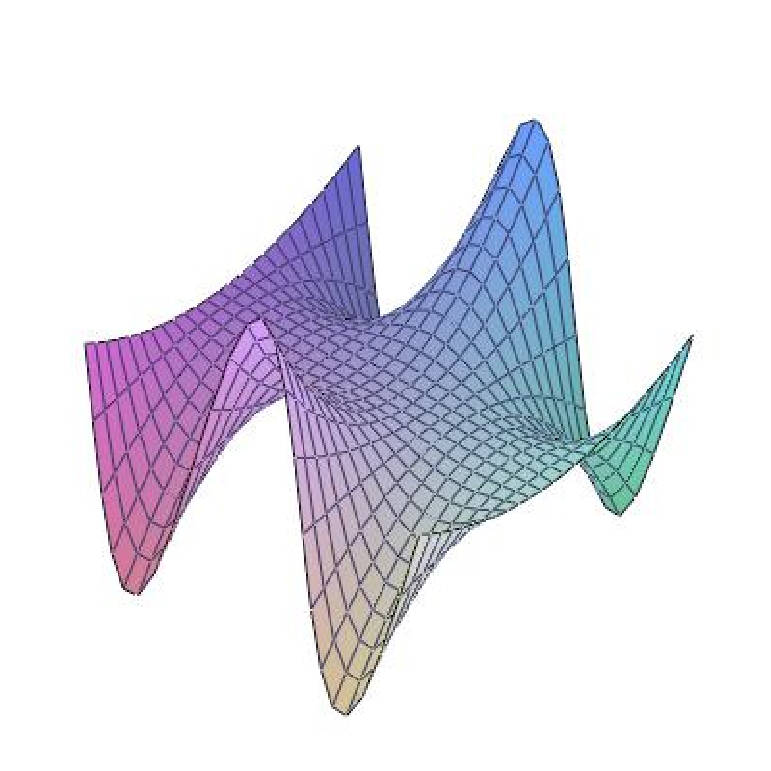
\includegraphics[scale=0.35]{grafica10.jpg}
\caption{Gráfica de $x^2\cdot cos(y)$}\label{cap6f1}
\end{figure}

\chapter{Tablas}

\section{Tabla de verdad}

En la tabla \ref{tab:cap7t1} podemos ver la tabla de verdad $p \rightarrow q$:

\begin{table}[ht]
	\caption{Tabla de verdad $p \rightarrow q$}
	\begin{center}
		\begin{tabular}{|c|c|c|} \hline
			$p$ & $q$ & $p \rightarrow q$\\\hline
			0 & 0 & 1 \\
			0 & 1 & 1 \\
			1 & 0 & 0 \\
			1 & 1 & 1 \\\hline
		\end{tabular}
	\end{center}
	\label{tab:cap7t1}
\end{table}

\chapter{Bibliográfia con \LaTeX{}}

\section{El entorno \textit{thebibliography}}

Existen varias formas de incluir citas bibliográficas en un 
documento de \LaTeX{}. Una de ellas consiste en incluir las
citas al final del documento, en una sección como la siguiente:

%\begin{thebibliography}{99}
%bibitem{expresion"Llave o identificador"}Información del documento
%cite{xpresion"Llave o ident} usado en el bibitem
\begin{verbatim}
\begin{thebibliography}{99}

\bibitem{spivakCalc} Spivak, Michael; Calculus; Reverte; 1996.

\bibitem{Lamport} Lamport, L.; \LaTeX{}; Addison-Wesley. 1996.

\end{thebibliography}
\end{verbatim}

Una vez incluida esta bibliografía, podemos hacer referencia a
una de las entradas mediante la siguiente expresión:

\begin{verbatim}
... el teorema del valor medio se puede consultar en
 \cite{spivakCalc} ... y \cite{Lamport} incluye un capitulo sobre
 como insertar gráficas en \LaTeX{} ...
\end{verbatim}


\section{Citas bibliográficas con Bib\TeX{}}

Otra forma más recomendable de incluir citas bibliográficas es
mediante el uso de Bib\TeX{}. En este caso es necesario crear
una ``\textit{base de datos}'' en un archivo de texto con 
extensión \textbf{.bib}, haciendo uso de la siguiente estructura:

\begin{verbatim}
@tipoDeCita{Llave,
	propiedad1={valor1},
	propiedad2={valor2},
	...
}
\end{verbatim}

En esta estructura, la \emph{Llave} es la expresión con la cual 
se hará referencia a una cita y en las propiedades se incluyen
los diferentes datos de ésta, tales como autor, año, páginas,
capítulo, abstract, entre otras \footnote{En la sección A.1
se incluyen algunas de las propiedades permitidas.}.

El \emph{tipoDeCita} indica en que clase de documento se incluirá
\footnote{La sección A.2 incluye algunos de los tipos
aceptados.}.

Este archivo debe estar ubicado en el mismo directorio en el que
se encuentra nuestro archivo \textbf{.tex}.

Una vez creada la base de datos, ésta puede ser incluida en el
documento mediante las siguientes instrucciones:

\begin{verbatim}
\bibliographystyle{Estilo}
\bibliography{basededatos1[,basededatos2,...]}
\end{verbatim}

Donde \emph{Estilo} indica el formato en el que se incluirán las
citas de la bibliografía y \emph{basededatosX} indica el archivo
o archivos de los cuales se tomarán los datos de las citas.

Algunos de los estilos más usados son: \emph{plain},
\emph{apalike}, \emph{alpha}, \emph{abbrv} y \emph{unsrt}.

Por ejemplo, las citas incluidas al inicio del apéndice se 
pueden incluir en un archivo \textbf{mibiblio.bib}, en el
siguiente formato:

\begin{verbatim}
@book{spivakCalc,
author="Spivak, Michael",
title="Calculus",
editor="Reverte",
year="1996",
pages="944"
}

@book{Lamport,
author="Leslie Lamport",
title="\LaTeX",
editor="Addison-Wesley",
year="1996"
}
\end{verbatim}

A continuación incluimos las siguientes instrucciones para 
insertar las citas:

\begin{verbatim}
\bibliographystyle{amsplain}
\bibliography{mibiblio}
\end{verbatim}

En este caso hacemos uso del estilo de la \emph{American 
Mathematical Society}. Con este estilo las citas se ordenan
alfabéticamente y se colocan etiquetas numéricas a cada una
de ellas.

La forma de incluir las citas es por medio del comando \textbackslash cite\{\}.
Por ejemplo:

\begin{verbatim}
Consulte ~\cite{Lamport} para conocer algo de \LaTeX{}
\end{verbatim}

Además, cuando se hace uso de este método, es necesario compilar nuestro
documento de la siguiente forma

\begin{verbatim}
pdflatex miDocumento.tex
bibtex miDocumento.tex
pdflatex miDocumento.tex
pdflatex miDocumento.tex
\end{verbatim}

Una de las ventajas de manejar la bibliografía de esta manera es
que solamente se incluiran las entradas citadas en el documento.

%Los capitulos o  secciones despues de \appendix seran apendices
\appendix

\chapter[Apendice A. Bib\TeX{}]{Bib\TeX{}}

\section{Propiedades soportadas}

Algunas de las propiedades soportadas por Bib\TeX{} son:

\begin{tabular}{llll}
address & abstract & author & booktitle \\
chapter & contents & copyright & crossref \\
edition & editor & howpublished & institution \\
ISBN & ISSN & journal & key \\
keywords & language & month & note \\
number & organization & pages & publisher \\
school & series & title &url \\
volume & year & & 
\end{tabular}

\newpage

\section{Tipos de citas}

Algunos de los tipos de citas válidos en los archivos de 
\emph{bases de datos} de Bib\TeX{} son:

\begin{tabular}{lll}
article & book & booklet \\
conference & inbook & incollection \\
inproceedings & manual & mastersthesis \\
misc & other & phdthesis \\
proceedings & techreport & unpublished
\end{tabular}

Consulte \cite{Lamport} para aprender algo de \LaTeX{}.

%\bibliographystyle{plain}
%\bibliography{mibiblio}

\begin{thebibliography}{99}

\bibitem{spivakCalc} Spivak, Michael; Calculus; Reverte; 1996.

\bibitem{Lamport} Lamport, L.; \LaTeX{}; Addison-Wesley. 1996.

\end{thebibliography}

\end{document}
